\documentclass[11pt]{article}

\usepackage[a4paper,margin=1in]{geometry}
\usepackage{amsmath,amssymb,amsthm,mathtools}
\usepackage{bm}
\usepackage{booktabs}
\usepackage{enumitem}
\usepackage{graphicx}
\usepackage{microtype}
\usepackage[hidelinks]{hyperref}
\hypersetup{
  pdftitle={Exact Robust Local Approximation of Graph Smoothers under Hidden-Network Completions},
  pdfauthor={Anonymous working draft}
}

\newtheorem{theorem}{Theorem}
\newtheorem{corollary}[theorem]{Corollary}
\theoremstyle{definition}
\newtheorem{definition}[theorem]{Definition}
\newtheorem{example}[theorem]{Example}
\theoremstyle{remark}
\newtheorem{remark}[theorem]{Remark}

\newcommand{\R}{\mathbb R}
\newcommand{\Sph}{\mathbb S}
\newcommand{\one}{\mathbf 1}
\newcommand{\conv}{\operatorname{conv}}
\newcommand{\cl}{\operatorname{cl}}
\newcommand{\diag}{\operatorname{diag}}
\newcommand{\tr}{\operatorname{tr}}
\newcommand{\dist}{\operatorname{dist}}
\newcommand{\supp}{\operatorname{supp}}
\newcommand{\rank}{\operatorname{rank}}
\newcommand{\cX}{\mathcal X}
\newcommand{\cP}{\mathcal P}
\newcommand{\cQ}{\mathcal Q}
\newcommand{\cE}{\mathcal E}
\newcommand{\cA}{\mathcal A}
\newcommand{\fG}{\mathfrak G}
\newcommand{\ip}[2]{\left\langle #1,#2\right\rangle}
\newcommand{\norm}[1]{\left\lVert #1\right\rVert}
\newcommand{\abs}[1]{\left\lvert #1\right\rvert}

\title{Exact Robust Local Approximation of Graph Smoothers\\
under Hidden-Network Completions}
\author{Anonymous working draft}
\date{September 2026}

\begin{document}
\maketitle

\begin{abstract}
We study a local linear approximation problem for graph-regularized state
smoothing when only a labeled boundary of the network is known.  A completion
may add hidden vertices, arbitrary undirected cycles, and arbitrary
nonnegative edge weights.  For at most $h$ unit-grounded hidden vertices, we
identify the exact closed convex hull of every visible principal block of
$(I+L)^{-1}$ by set partitions and integer hidden-budget allocations.  We
characterize all exposed vertices, give connected maximum-degree-two path
converses, and prove an exact $q/(q+h)$ operator-Hausdorff convergence rate to
an unbounded partial-partition polytope.  Keeping all hidden-input columns, we
then reduce every finite-budget Schatten-norm worst case to finitely many
canonical errors.  In the unbounded limit the same reduction holds exactly
for Schatten exponents at least two, and a two-vertex example proves that the
threshold is sharp.  The spectral problem with any semidefinite-representable
local-rule constraint is consequently a finite, necessary-and-sufficient SDP.
The argument uses the established random-forest mean-projection identity as a
tool; we do not claim that identity as new.
\end{abstract}

\section{Introduction}

Consider the graph-regularized estimator
\begin{equation}
  \widehat x_G(y)
  =\arg\min_x\left\{
       \frac12\norm{x-y}_2^2
       +\frac12\sum_{\{i,j\}\in E}w_{ij}(x_i-x_j)^2
    \right\}
  =(I+L_G)^{-1}y .
  \label{eq:smoother}
\end{equation}
Only $q$ visible vertices, called \emph{ports}, are available to a local
algorithm.  The remaining topology and inputs are hidden.  The goal is not to
recover a particular unknown topology, but to choose one common port-only
linear map that is valid for every admissible completion.

This question has an infinite adversarial description: the hidden vertex
count, graph topology, cycles, edge weights, and hidden input coordinates all
vary.  Our result eliminates that description exactly.  With a finite hidden
budget, the scenarios are indexed by a full partition of the ports and an
integer allocation of hidden vertices to its blocks.  Without a budget, they
are indexed by partial partitions.  Both families are fixed-parameter in the
boundary size; neither is polynomial in $q$.

The proof begins with the matrix-forest/random-spanning-forest representation
of a grounded Laplacian inverse.  This representation and its more general
determinantal mean-projection form are established results
\cite{chebotarev1997,pilavci2021,derezinski2020,kassel2023}.  Our focus is the
image of all hidden completions at the ports, its exact finite-budget geometry,
the matching low-degree network realization, and the resulting robust local
design problem.

The scope is deliberately narrow.  The main model is scalar, undirected,
unit-grounded, and has nonnegative edge weights.  We do not identify the
smoother error in \eqref{eq:smoother} with the measurement-noise MSE of a
general WLS or Kalman estimator.  Directed, signed, block-valued, and nonlinear
extensions are outside the claims of this paper.

\begin{figure}[t]
  \centering
  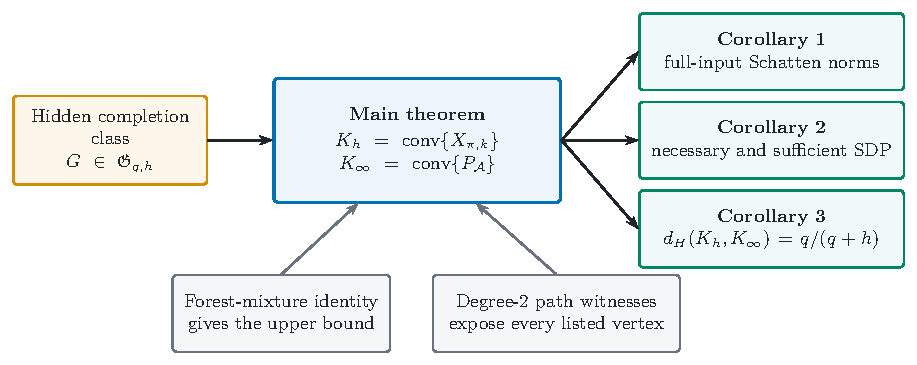
\includegraphics[width=\linewidth]{figures/tikz/theorem_structure.pdf}
  \caption{Logical structure of the result.  The forest-mixture identity
  supplies the upper inclusion, while connected maximum-degree-two paths
  expose the listed vertices and give the converse.  The exact completion
  hulls then imply the three application corollaries.}
  \label{fig:theorem-structure}
\end{figure}

\section{Completion model and local rules}

Let $\Gamma=\{1,\ldots,q\}$ be the labeled port set.  A finite completion is a
weighted undirected graph
\[
  G=(V,E,w),\qquad V=\Gamma\mathbin{\dot\cup}Z,\qquad w_e\geq0,
\]
where $Z$ is a set of hidden vertices and $L_G$ is the weighted graph
Laplacian.  All vertices have unit grounding.  Define
\begin{equation}
  T_G=(I_{q+|Z|}+L_G)^{-1},\qquad
  E_\Gamma=[I_q\ \ 0],\qquad
  X_G=E_\Gamma T_GE_\Gamma^T .
  \label{eq:TG-XG}
\end{equation}
For $h\in\mathbb Z_+$, let $\fG_{q,h}$ contain every such completion with
$|Z|\leq h$, with no restriction on cycles or finite edge conductances.  Let
$\fG_{q,\infty}=\bigcup_{h\geq0}\fG_{q,h}$.  We also use the subclasses with
exactly $h$ hidden vertices and with a connected underlying graph.

All closures below are in the finite-dimensional space $\Sph^q$ with the
operator-norm topology.  Thus an equality involving a closure describes
limiting high-conductance or weak-link graphs; it does not assert that every
boundary point is attained at finite conductance.  Likewise, $\sup_G$ always
means a supremum over the stated completion class, rather than a maximum on a
fixed topology.

Fix an output matrix $C\in\R^{d\times q}$.  The centralized port output on a
full input $y\in\R^{q+|Z|}$ is $CE_\Gamma T_Gy$.  A common local linear rule can
read only $E_\Gamma y$ and has the form
\begin{equation}
  Q E_\Gamma y,\qquad Q\in\cQ_{\rm loc}\subseteq\R^{d\times q}.
  \label{eq:local-rule}
\end{equation}
The full-input error operator is
\begin{equation}
  \cA_G(Q)=CE_\Gamma T_G-QE_\Gamma
  \in\R^{d\times(q+|Z|)}.
  \label{eq:full-error}
\end{equation}
The word ``common'' is essential: $Q$ cannot depend on the hidden completion.

A convenient general representation of local implementability is
\begin{equation}
  Q(\theta)=Q_0+\sum_{a=1}^s\theta_aB_a,
  \qquad \theta\in\Theta,
  \label{eq:affine-rule}
\end{equation}
where $\Theta$ is closed and semidefinite representable.  Fixed zero patterns
are obtained by omitting coordinate matrices $B_a$.  If output row $i$ is
located at port $o(i)$ in a visible communication graph $H$, an $r$-round rule
imposes
\[
  Q_{ij}=0\quad\text{when}\quad \dist_H(o(i),j)>r.
\]
Equating coefficients of selected $B_a$'s gives shared-coefficient or
shared-opcode rules.  These restrictions may be intersected with unbiasedness,
row-sum, or other affine constraints.  No particular choice of
$\cQ_{\rm loc}$ is needed for the geometric result.

\subsection{Finite and unbounded scenario sets}

For a full set partition $\pi$ of $\Gamma$ and an allocation
$k=(k_B)_{B\in\pi}\in\mathbb Z_+^{|\pi|}$ with
$|k|_1=\sum_Bk_B\leq h$, set
\begin{equation}
  X_{\pi,k}
  =\sum_{B\in\pi}\frac{\one_B\one_B^T}{|B|+k_B},
  \qquad
  \cX_{q,h}=\{X_{\pi,k}:\pi\vdash\Gamma,\ |k|_1\leq h\},
  \qquad K_h=\conv\cX_{q,h}.
  \label{eq:finite-scenarios}
\end{equation}
Here $\one_B$ is the indicator of $B$ in $\R^q$.  Every
$X\in\cX_{q,h}$ is a positive contraction, but it is generally not a
projection.  We write $\pi\vdash U$ to mean that $\pi$ is a set partition of
$U$.

For a subset $U\subseteq\Gamma$ and a partition $\pi$ of $U$, define
\begin{equation}
  P_{\pi,U}=\sum_{B\in\pi}P_B,
  \qquad P_B=\frac{\one_B\one_B^T}{|B|},
  \qquad
  \cP_q^\partial=\{P_{\pi,U}:U\subseteq\Gamma,\ \pi\vdash U\},
  \qquad K_\infty=\conv\cP_q^\partial .
  \label{eq:partial-scenarios}
\end{equation}
The empty active set gives $P=0$.  Every member of $\cP_q^\partial$ is an
orthogonal projection.  Joining all inactive ports to one cemetery symbol
gives a bijection with partitions of $q+1$ elements, so
$|\cP_q^\partial|=B_{q+1}$, where $B_j$ is a Bell number.

\section{Exact completion geometry}

We now state the single geometric theorem used throughout the paper.  It
includes the finite physical model and its unbounded sharp limit.

\begin{theorem}[Finite-budget completion hull and partial-partition limit]
\label{thm:main}
For every $q\geq1$ and $h\geq0$, the following statements hold.

\begin{enumerate}[label=\textup{(\roman*)},leftmargin=2.1em]
\item The finite-budget port image has the exact closed convex hull
\begin{equation}
  \cl\conv\{X_G:G\in\fG_{q,h}\}=K_h.
  \label{eq:finite-hull}
\end{equation}
The same right-hand side is obtained with exactly $h$ hidden vertices and
with connected completions.  Every $X_{\pi,k}\in\cX_{q,h}$ is approached by
a sequence of connected weighted paths, hence by graphs of maximum degree at
most two.

\item The parameterization in \eqref{eq:finite-scenarios} has no repetitions,
and its cardinality is
\begin{equation}
  N(q,h)=\sum_{s=1}^q S(q,s)\binom{h+s}{s},
  \label{eq:candidate-count}
\end{equation}
where $S(q,s)$ is a Stirling number of the second kind.  If $h\geq1$, the
vertices of $K_h$ are exactly
\begin{equation}
  \operatorname{vert}(K_h)
  =\{X_{\pi,0}:\pi\vdash\Gamma\}
   \cup
   \{X_{\pi,k}:|k|_1=h\},
  \label{eq:finite-vertices}
\end{equation}
and every listed vertex is exposed.  Consequently,
\begin{equation}
  N_{\rm vert}(q,h)
  =\sum_{s=1}^q S(q,s)
       \left[1+\binom{h+s-1}{s-1}\right].
  \label{eq:vertex-count}
\end{equation}
For $h=0$, all $B_q$ full-partition projections are exposed vertices.

\item The hulls satisfy $K_h\subseteq K_\infty$ and
\begin{equation}
  \cl\conv\{X_G:G\in\fG_{q,\infty}\}=K_\infty.
  \label{eq:unbounded-hull}
\end{equation}
Every $P\in\cP_q^\partial$ is an exposed vertex of $K_\infty$ and is
approached by connected weighted paths.

\item With operator norm as the metric, the convergence is exact for every
$q$ and $h$:
\begin{equation}
  d_H^{\rm op}(K_h,K_\infty)=\frac{q}{q+h}.
  \label{eq:hausdorff}
\end{equation}
\end{enumerate}
\end{theorem}

\begin{proof}
\textbf{Forest-mixture upper bound.}
Give $G$ an arbitrary orientation and write $L_G=AA^T$, where the column for
edge $e=(u,v)$ is $\sqrt{w_e}(e_u-e_v)$.  The established $L$-ensemble
mean-projection identity gives
\begin{equation}
  (I+AA^T)^{-1}
  =\mathbb E\,P_{\ker A_S^T},
  \qquad
  \Pr(S)=\frac{\det(A_S^TA_S)}{\det(I+A^TA)},
  \label{eq:dpp-identity}
\end{equation}
with the empty determinant equal to one
\cite{derezinski2020,kassel2023}.  A dependent edge set has zero probability;
for an incidence matrix, the remaining sets are precisely forests.  If the
components of such a forest are $D$, then
\begin{equation}
  P_{\ker A_S^T}=\sum_D\frac{\one_D\one_D^T}{|D|}.
  \label{eq:forest-projector}
\end{equation}
For every component meeting $\Gamma$, put $B=D\cap\Gamma$ and
$k_B=|D\cap Z|$.  These nonempty $B$'s form a full partition of $\Gamma$,
$\sum_Bk_B\leq|Z|\leq h$, and the port principal block of
\eqref{eq:forest-projector} is exactly $X_{\pi,k}$.  Hidden-only components
consume budget but contribute no port entry.  Taking the port block in
\eqref{eq:dpp-identity} proves
$X_G\in K_h$ and hence the upper inclusion in \eqref{eq:finite-hull}.  This is
the only place where the known forest-mixture identity is used.

\textbf{Connected path converse.}
Fix $(\pi,k)$.  For each $B\in\pi$, arrange its ports and $k_B$ hidden
vertices into one path segment.  If exactly $h$ hidden vertices are required,
arrange the unused vertices in additional hidden-only segments.  Give every
within-segment edge conductance $t$.  At zero conductance between segments,
\begin{equation}
  (I+tL_F)^{-1}\longrightarrow P_{\ker L_F}
  \quad(t\to\infty),
  \label{eq:high-conductance}
\end{equation}
whose port block is $X_{\pi,k}$.  Concatenate all segments at their endpoints
with positive bridge conductances $\varepsilon$.  The resulting finite graph
is a connected path.  For each sufficiently large $t_n$, continuity of the
inverse permits a sufficiently small $\varepsilon_n>0$ so that the same limit
is obtained.  This diagonal sequence proves the reverse inclusion, all three
completion-class variants, and the degree-two assertion.  Closure is in
general necessary: $T_G\succ0$ at finite conductance, whereas many scenario
matrices are singular.

\textbf{Counting and absence of repetitions.}
For a partition with $s$ blocks, the number of weak allocations with total at
most $h$ is $\binom{h+s}{s}$.  Summing over the $S(q,s)$ partitions proves
\eqref{eq:candidate-count}.  The positive off-diagonal pattern of a scenario
recovers its blocks.  On a recovered block $B$, the common value
$1/(|B|+k_B)$ recovers $k_B$, so no two parameters give the same matrix.

\textbf{Finite exposed vertices.}
Suppose $0<|k|_1<h$ and choose $B$ with $k_B>0$.  Holding all other
allocations fixed, set
\[
  K=h-\sum_{D\neq B}k_D>k_B.
\]
Because $1/(|B|+k_B)$ lies strictly between $1/|B|$ and
$1/(|B|+K)$, the scenario is a strict convex combination of the two feasible
scenarios obtained by replacing $k_B$ with $0$ and $K$.  It is not a vertex.

For $k=0$, $X_{\pi,0}=P_\pi$ is an orthogonal projection.  The functional
$X\mapsto\ip{2P_\pi-I}{X}$ uniquely maximizes at $P_\pi$ over the entire
positive-contraction interval $0\preceq X\preceq I$: indeed,
\[
 \ip{2P_\pi-I}{X}
 =\tr(P_\pi XP_\pi)-\tr((I-P_\pi)X(I-P_\pi))
 \leq\rank P_\pi,
\]
and equality forces the two diagonal compressions to be $P_\pi$ and zero;
positivity of both $X$ and $I-X$ then forces the cross terms to vanish.  Thus
$X=P_\pi$, which exposes it in $K_h$.

It remains to expose a target $(\pi,k^*)$ with $|k^*|_1=h$.  Define a symmetric
matrix $H_\pi$ by
\[
 (H_\pi)_{ii}=-(|B|-1)\quad(i\in B),
 \qquad
 (H_\pi)_{ij}=
 \begin{cases}
  1,&i\neq j\text{ in the same }B\in\pi,\\
  -1,&i,j\text{ in different blocks of }\pi.
 \end{cases}
\]
If $S\neq\varnothing$ and $r_B=|S\cap B|$, then
\begin{equation}
  \one_S^TH_\pi\one_S
  =\sum_{B\in\pi}r_B(r_B-|B|)
   -2\sum_{B<D}r_Br_D\leq0,
  \label{eq:partition-separator}
\end{equation}
with equality exactly when $S$ is one target block.  Hence
$\ip{H_\pi}{X_{\pi,k}}=0$ for the target partition and is strictly negative
for every other partition.

On each target block choose a constant matrix $A_B$ satisfying
$\one_B^TA_B\one_B=-\gamma_B$, where
$\gamma_B=(|B|+k_B^*)^2$, and put all cross-block entries of $A$ to zero.
For the target partition,
\begin{equation}
  f(k)=\ip{A}{X_{\pi,k}}
      =-\sum_B\frac{\gamma_B}{|B|+k_B}.
  \label{eq:allocation-exposer}
\end{equation}
The gain from the $(r+1)$st hidden vertex in block $B$ is
\[
  \Delta_B(r)
  =\frac{\gamma_B}{(|B|+r)(|B|+r+1)}.
\]
Selected increments have gain greater than one and unselected increments have
gain less than one.  Hence $k^*$ uniquely maximizes
\eqref{eq:allocation-exposer} under $|k|_1\leq h$: any different feasible
allocation omits a selected increment or replaces one by a strictly smaller
unselected increment.  Finiteness then implies
that $MH_\pi+A$ exposes the target for all sufficiently
large $M$.  This proves \eqref{eq:finite-vertices}; stars-and-bars gives
\eqref{eq:vertex-count}.

\textbf{Partial-partition limit and exposedness.}
Write each finite scenario as
\[
  X_{\pi,k}=\sum_{B\in\pi}\alpha_BP_B,
  \qquad \alpha_B=\frac{|B|}{|B|+k_B}\in(0,1].
\]
Independently retain block $B$ with probability $\alpha_B$.  The resulting
random sum is a partial-partition projection with expectation $X_{\pi,k}$.
Therefore $K_h\subseteq K_\infty$.

Conversely, fix $P_{\pi,U}$ and let $I=\Gamma\setminus U$.  If $I\neq
\varnothing$, append $I$ as one full-partition block and allocate all $h$
hidden vertices to it.  This gives
\begin{equation}
  X_h=P_{\pi,U}+\frac{|I|}{|I|+h}P_I\longrightarrow P_{\pi,U}.
  \label{eq:partial-approximation}
\end{equation}
If $I$ is empty, take $X_h=P_{\pi,U}$.  Applying the connected path
construction above and taking a diagonal sequence proves
\eqref{eq:unbounded-hull} and its path converse.  This construction also
controls the omitted columns: in the fused component containing $I$, the
squared Euclidean norm of each inactive port row is $1/(|I|+h)$, whereas the
active components contain no hidden vertices.  After zero padding, the full
port rows therefore converge to $[P_{\pi,U}\ \ 0]$.  For distinct orthogonal
projections $P,P'\in\cP_q^\partial$,
\begin{equation}
  \ip{2P-I}{P'}
  =\tr P-\norm{P-P'}_F^2
  <\tr P=\ip{2P-I}{P},
  \label{eq:partial-exposed}
\end{equation}
so every partial scenario is exposed.

\textbf{Exact Hausdorff distance.}
Equation \eqref{eq:partial-approximation} gives
$\norm{X_h-P_{\pi,U}}_2\leq q/(q+h)$.  Extending this approximation from
vertices to their convex combinations proves the upper bound in
\eqref{eq:hausdorff}.  For the reverse bound, let
$u=\one_\Gamma/\sqrt q$.  Every finite scenario satisfies
\begin{equation}
 u^TX_{\pi,k}u
 =\frac1q\sum_{B\in\pi}\frac{|B|^2}{|B|+k_B}
 \geq\frac1q\frac{(\sum_B|B|)^2}{\sum_B(|B|+k_B)}
 \geq\frac{q}{q+h}.
 \label{eq:hausdorff-lower}
\end{equation}
The inequality persists under convex combinations, while the one-block
scenario with $k=h$ has operator norm exactly $q/(q+h)$.  Since
$0\in K_\infty$, its distance to $K_h$ is exactly this value.  The proof is
complete.
\end{proof}

\section{Full hidden-input error and the Schatten boundary}

For $X\in\cX_{q,h}$ define the canonical error
\begin{equation}
  \cE_Q(X)
  =\left[CX-Q\ ,\ C(X-X^2)^{1/2}\right]
  \in\R^{d\times2q}.
  \label{eq:canonical-error}
\end{equation}
The square root exists because $0\preceq X\preceq I$.  Its second block is
not optional: it records exactly the hidden-input energy absent from the port
principal block.

\begin{corollary}[Exact full-input Schatten reductions]
\label{cor:schatten}
Fix $C\in\R^{d\times q}$ and $Q\in\R^{d\times q}$.

\begin{enumerate}[label=\textup{(\roman*)},leftmargin=2.1em]
\item For every finite $h$ and every $1\leq s\leq\infty$,
\begin{equation}
  \sup_{G\in\fG_{q,h}}\norm{\cA_G(Q)}_{S_s}
  =\max_{X\in\cX_{q,h}}\norm{\cE_Q(X)}_{S_s}.
  \label{eq:finite-schatten}
\end{equation}
The same equality holds for every unitarily invariant matrix norm.

\item If $2\leq s\leq\infty$, the finite maximum in
\eqref{eq:finite-schatten} may be restricted to the vertices in
\eqref{eq:finite-vertices}.  In the unbounded model,
\begin{equation}
  \sup_{G\in\fG_{q,\infty}}\norm{\cA_G(Q)}_{S_s}
  =\max_{P\in\cP_q^\partial}\norm{CP-Q}_{S_s}.
  \label{eq:unbounded-schatten}
\end{equation}

\item The exponent threshold in \eqref{eq:unbounded-schatten} is sharp over
the Schatten family: a universal equality for all $C,Q$ and all completions
holds if and only if $s\geq2$.
\end{enumerate}
\end{corollary}

\begin{proof}
For the forest random projection $\widehat P=P_{\ker A_S^T}$ in
\eqref{eq:dpp-identity}, put
$A_{\widehat P}=CE_\Gamma\widehat P-QE_\Gamma$.  Convexity of any matrix norm
gives
\[
  \norm{\cA_G(Q)}
  =\norm{\mathbb E A_{\widehat P}}
  \leq\mathbb E\norm{A_{\widehat P}}.
\]
With $X=E_\Gamma\widehat PE_\Gamma^T$ and $\widehat P^2=\widehat P$, direct
multiplication gives the key affine Gram identity
\begin{align}
  A_{\widehat P}A_{\widehat P}^T
  &=CXC^T-CXQ^T-QXC^T+QQ^T \notag\\
  &=(CX-Q)(CX-Q)^T+C(X-X^2)C^T
   =\cE_Q(X)\cE_Q(X)^T.
  \label{eq:gram-identity}
\end{align}
Thus $A_{\widehat P}$ and $\cE_Q(X)$ have the same singular values.  Every
forest compression is in $\cX_{q,h}$, proving the upper bound in
\eqref{eq:finite-schatten}.  The connected high-conductance path sequence in
Theorem~\ref{thm:main} makes the full projection rows, and hence the Gram
matrix in \eqref{eq:gram-identity}, converge to each candidate value.  This
proves the reverse inequality for all unitarily invariant norms.

For finite $2\leq s<\infty$, the $s$th power of the scenario loss is
\[
  X\longmapsto\tr\left(M_Q(X)^{s/2}\right),
  \qquad M_Q(X)=CXC^T-CXQ^T-QXC^T+QQ^T.
\]
It is convex on positive semidefinite matrices \cite{bhatia1997}, and $M_Q$ is affine in $X$.
For $s=\infty$, use the convex function
$\lambda_{\max}(M_Q(X))$.  A convex function on $K_h$ has a maximizer among
its vertices, proving the pruning statement.  Every finite scenario belongs
to $K_\infty=\conv\cP_q^\partial$; affinity of $M_Q$ and the same convexity
bound its loss by the largest partial-scenario loss.  Conversely, every
partial scenario is approached by the path sequence in
Theorem~\ref{thm:main}, and $P^2=P$ makes its canonical error
$[CP-Q\ \ 0]$.  This proves \eqref{eq:unbounded-schatten}.

To prove sharpness, take one port, one hidden vertex, and let their connecting
conductance tend to infinity.  The full projection tends to
\[
  \widehat P=\frac12\begin{bmatrix}1&1\\1&1\end{bmatrix}.
\]
Choose
$C=(1,1)^T$ and $Q=(1,0)^T$.  The two partial scenarios $P=0,1$ have error
vectors $-Q$ and $C-Q$, both of Schatten norm one.  The full limiting error is
\[
  \begin{bmatrix}-1/2&1/2\\1/2&1/2\end{bmatrix},
\]
whose two singular values are $1/\sqrt2$.  Its Schatten-$s$ norm is
$2^{1/s-1/2}>1$ exactly when $1\leq s<2$.  The positive result includes
$s=2$, so the boundary is exact.
\end{proof}

For $s<2$, equation \eqref{eq:finite-schatten} remains valid, but an
unexposed finite candidate cannot be deleted merely because it is not a
vertex of $K_h$: the full-input risk need not be convex in $X$.

\section{Lossless local-rule SDP}

Let $\mathcal V_{q,h}$ denote the finite vertex set in
\eqref{eq:finite-vertices}, with all full partitions used when $h=0$.  The
following certificate directly supports zero-pattern, $r$-hop, and shared
coefficient constraints through \eqref{eq:affine-rule}.

\begin{corollary}[Necessary-and-sufficient spectral SDP]
\label{cor:sdp}
Assume $\cQ_{\rm loc}$ is nonempty, closed, and semidefinite representable.
For the finite completion class, the squared optimal radius is exactly the
optimal value of
\begin{equation}
\begin{aligned}
 \underset{Q\in\cQ_{\rm loc},\ \rho\geq0}{\operatorname{minimize}}
 &\quad \rho\\
 \text{subject to}
 &\quad
 \begin{bmatrix}
  \rho I_d-CXC^T+CXQ^T+QXC^T & Q\\
  Q^T&I_q
 \end{bmatrix}\succeq0,
 \qquad X\in\mathcal V_{q,h}.
\end{aligned}
\label{eq:finite-sdp}
\end{equation}
Equivalently, for any prescribed $\varepsilon\geq0$, a common local $Q$ with
$\sup_{G\in\fG_{q,h}}\norm{\cA_G(Q)}_2\leq\varepsilon$ exists if and only if
\eqref{eq:finite-sdp} is feasible with $\rho=\varepsilon^2$.

For the unbounded class, the optimal radius is exactly the optimal value of
\begin{equation}
\begin{aligned}
 \underset{Q\in\cQ_{\rm loc},\ \tau\geq0}{\operatorname{minimize}}
 &\quad \tau\\
 \text{subject to}
 &\quad
 \begin{bmatrix}
  \tau I_d&CP-Q\\
  (CP-Q)^T&\tau I_q
 \end{bmatrix}\succeq0,
 \qquad P\in\cP_q^\partial.
\end{aligned}
\label{eq:unbounded-sdp}
\end{equation}
Both optima are attained.  There is no completion-scenario relaxation gap.
\end{corollary}

\begin{proof}
For fixed $X$, the Schur complement of the lower-right identity in
\eqref{eq:finite-sdp} is
\[
  \rho I_d-
  \left(CXC^T-CXQ^T-QXC^T+QQ^T\right)\succeq0.
\]
By \eqref{eq:gram-identity}, this is equivalent to
$\norm{\cE_Q(X)}_2^2\leq\rho$.  Corollary~\ref{cor:schatten} and exact vertex
pruning prove necessity and sufficiency.  For a partial projection, the
hidden block in \eqref{eq:canonical-error} vanishes; the standard rectangular
spectral-norm epigraph gives \eqref{eq:unbounded-sdp}
\cite{boyd2004}.  The scenario families
are finite.  Moreover $X=I$ is a finite scenario and $P=0$ is an unbounded
scenario, so bounded objective values bound $Q$; closedness gives attainment.
\end{proof}

The finite formulation uses $N_{\rm vert}(q,h)$ LMIs of order $d+q$.  The
unbounded formulation uses $B_{q+1}$ LMIs of the same order.  This is an exact
boundary-size fixed-parameter algorithm, not a polynomial-time claim in $q$.
The accompanying implementation enumerates restricted-growth set partitions,
weak integer compositions, and active scenarios, and it verifies the returned
$Q$ against every exact candidate after solving.

\section{Quantitative budget hierarchy}

Define the fixed-rule spectral radii
\[
  R_h(Q)=\sup_{G\in\fG_{q,h}}\norm{\cA_G(Q)}_2,
  \qquad
  R_\infty(Q)=\sup_{G\in\fG_{q,\infty}}\norm{\cA_G(Q)}_2.
\]

\begin{corollary}[Finite-budget convergence of certified risk]
\label{cor:rate}
For every fixed $C,Q$ and every $h\geq0$,
\begin{equation}
  0\leq R_\infty(Q)^2-R_h(Q)^2
  \leq
  \left(\norm{C}_2^2+2\norm{C}_2\norm{Q}_2\right)
  \frac{q}{q+h}.
  \label{eq:risk-rate}
\end{equation}
\end{corollary}

\begin{proof}
Let $g_Q(X)=\lambda_{\max}(M_Q(X))$, with $M_Q$ as in
\eqref{eq:gram-identity}.  Since $K_h\subseteq K_\infty$ and $g_Q$ is convex,
the left inequality follows from the exact scenario reductions.  For
$X,Y\in K_\infty$, Weyl's inequality and submultiplicativity give
\[
 |g_Q(X)-g_Q(Y)|
 \leq\norm{M_Q(X)-M_Q(Y)}_2
 \leq(\norm{C}_2^2+2\norm{C}_2\norm{Q}_2)\norm{X-Y}_2.
\]
Combine this Lipschitz bound with the exact Hausdorff distance
\eqref{eq:hausdorff}.
\end{proof}

\begin{figure}[t]
  \centering
  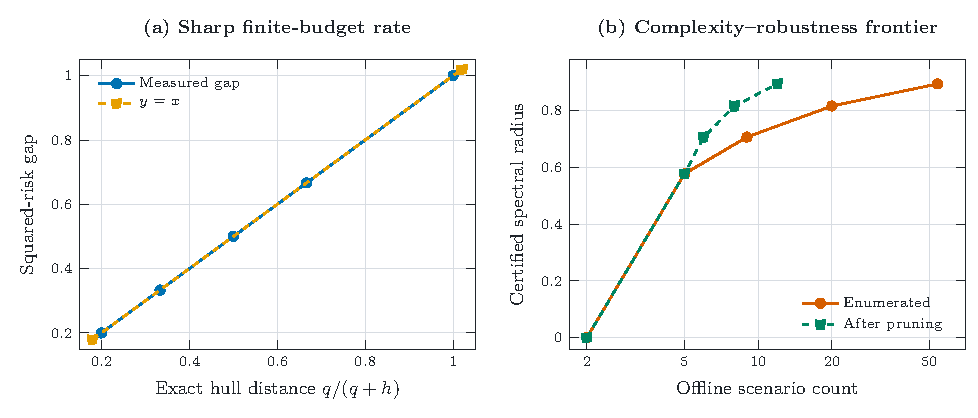
\includegraphics[width=\linewidth]{figures/tikz/budget_pareto.pdf}
  \caption{Finite hidden-budget hierarchy for the two-port fixed-rule audit.
  The measured finite-to-unbounded squared-risk gaps coincide numerically with
  the exact distance $q/(q+h)$.  Increasing the hidden budget increases both
  the certified radius and the offline scenario count; exact pruning deletes
  redundant LMIs without changing the radius.}
  \label{fig:budget-pareto}
\end{figure}

\section{Graph-smoothing examples and algorithmic meaning}

\subsection{A finite-budget gain that is not imposed by a protocol constraint}

Let $q=2$, $h=1$, and
$C=P_{\rm av}=\one\one^T/2$.  The five exact candidates are
\[
 I,\quad \diag(1/2,1),\quad \diag(1,1/2),\quad
 P_{\rm av},\quad \frac23P_{\rm av}.
\]
The unconstrained solution of \eqref{eq:finite-sdp} is
\begin{equation}
 Q_*=\frac23P_{\rm av},
 \qquad R_1^*=\frac{\sqrt2}{3}=0.471404\ldots .
 \label{eq:finite-example}
\end{equation}
Indeed, the five radii at this $Q$ are respectively
$1/3,\sqrt7/6,\sqrt7/6,1/3,\sqrt2/3$.  The last scenario has the unavoidable
hidden-input term
\[
 C\left(\frac23P_{\rm av}-\frac49P_{\rm av}\right)C^T
 =\frac29P_{\rm av},
\]
which proves optimality.  The unbounded optimum is $1/2$, so knowing $h=1$
reduces radius by $5.72\%$ and squared risk by $11.11\%$.  At $h=0$, the
choice $Q=C$ has zero error.

\subsection{Why a nontrivial unbounded design needs a genuine local rule}

If $Q$ is unrestricted, $P=0$ and $P=I$ imply
\[
 \max_{P\in\cP_q^\partial}\norm{CP-Q}_2\geq\frac12\norm C_2,
\]
while $Q=C/2$ attains equality for every orthogonal projection $P$.  Thus the
unbounded free-$Q$ problem has the transparent solution
$Q_*=C/2$, $R_\infty^*=\norm C_2/2$.  Communication sparsity or another real
protocol restriction is required for a substantive design tradeoff.

For a minimal shared-opcode example, take
\[
 C=\diag(1,2),\qquad \cQ_{\rm loc}=\{\alpha I_2:\alpha\in\R\}.
\]
The exact five-scenario problem gives
\begin{equation}
 \alpha_*=\frac43-\frac{2\sqrt{10}}{15}=0.911696\ldots,
 \qquad
 R_*=\frac{10+2\sqrt{10}}{15}=1.088304\ldots .
 \label{eq:shared-example}
\end{equation}
Dropping the connected partial scenario $P_{\rm av}$ instead gives the
incorrect answer $\alpha=1$, $R=1$: the robust radius is underestimated by
$8.83\%$.  This example also illustrates why the solver reports the active
scenario set rather than only the optimal matrix.

\begin{figure}[t]
  \centering
  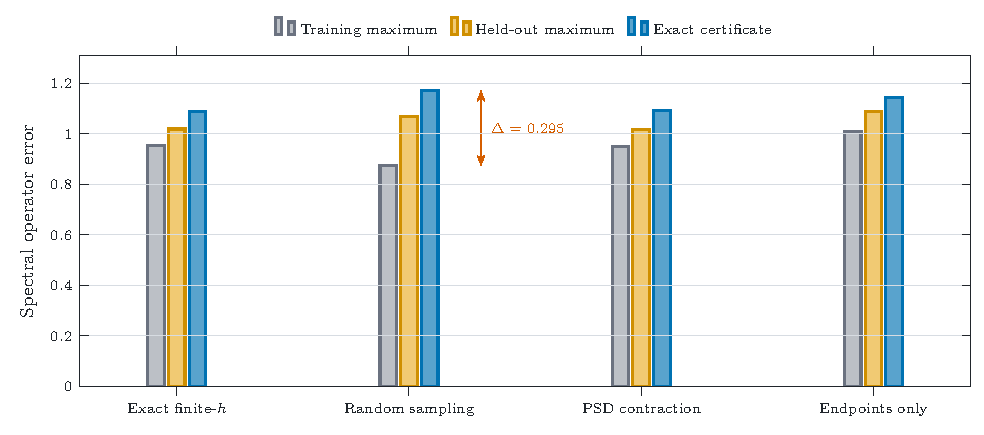
\includegraphics[width=\linewidth]{figures/tikz/certificate_sampling_failure.pdf}
  \caption{Certificate comparison for $q=3$, $h=2$, one-hop path support, and
  shared diagonal coefficients.  Physical training and held-out maxima do not
  certify the completion class.  The rule trained on 12 random completions
  understates its exact finite-budget worst case by $0.295$.  The plotted blue
  bars re-evaluate every returned rule on the exact finite scenario set.}
  \label{fig:certificate-failure}
\end{figure}

\subsection{Offline and online costs}

Scenario generation, conic model construction, and SDP solution are offline
design costs.  They depend exponentially on the port boundary but not on the
eventual hidden network size.  Once $Q$ is fixed, online estimation is simply
$QE_\Gamma y$.  Under an $r$-hop zero pattern its operational accounting can
therefore be kept separate: $r$ synchronous rounds, protocol-dependent message
and byte-hop counts, $\operatorname{nnz}(Q)$ multiply-adds per signal, and
storage proportional to $\operatorname{nnz}(Q)$.  These quantities are not
part of the mathematical radius and should be reported separately in
experiments.

\begin{figure}[t]
  \centering
  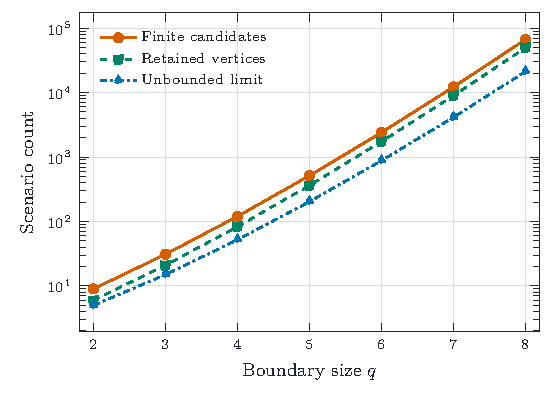
\includegraphics[width=0.58\linewidth]{figures/tikz/scenario_scaling.pdf}
  \caption{Exact scenario counts at hidden budget $h=2$.  Finite candidates,
  retained finite-hull vertices, and unbounded partial partitions all grow
  combinatorially with $q$.  The reduction is boundary-size fixed-parameter,
  not polynomial in the boundary size.}
  \label{fig:scenario-scaling}
\end{figure}

\section{Computational validation}

\subsection{Protocol and certificate audit}

We use two explicitly separated experiment tracks.  The theorem-matched track
optimizes a common port rule over the exact completion scenarios and measures
the full-input operator norm in \eqref{eq:full-error}.  The fixed-graph track
instead reveals one complete graph and compares graph-smoothing algorithms on
that instance.  Its empirical MSE is a graph-signal metric and is never labeled
as a general WLS or Kalman measurement-noise MSE.

The principal theorem-matched instance uses $q=3$, $h=2$,
$C=\diag(1,1.5,2)$, a one-hop path zero pattern, and one shared coefficient for
the three diagonal entries of $Q$.  The exact finite certificate is
$1.088304$.  A design trained on 12 random physical completions reports radius
$0.875273$, but exact re-evaluation gives $1.170691$, the gap displayed in
Figure~\ref{fig:certificate-failure}.  The safe
$0\preceq X\preceq I$ outer relaxation returns radius $1.122185$; the same
rule has exact finite risk $1.092846$, so the safety margin is conservative.
The endpoint-only NO-GO design reports approximately $1$ on its reduced set
but has exact finite risk $1.144123$.

Exact pruning reduces the finite model from 31 to 21 LMIs, a $32.3\%$
reduction.  The pruned and unpruned radii differ by only
$1.7\times10^{-9}$; on this smoke instance their total offline times are
$0.0405$ and $0.0526$ seconds, respectively.  At $q=8$ and $h=2$, generation
alone produces 66,491 candidates, 49,484 retained vertices, and 21,147
unbounded partial partitions.  This confirms the intended boundary-size
parameterization and also identifies its practical combinatorial limit.

For the optimized three-port rule, one explicit shortest-path unicast schedule
uses one synchronous round, four scalar-hops (32 byte-hops in double precision),
11 online FLOPs, and 100 bytes of sparse coefficient storage.  These numbers
describe an implementable schedule, not communication lower bounds.

\subsection{Fixed-graph local algorithms}

We next average over four 36-node weighted graphs: random cyclic, grid,
geometric, and small-world.  Each point uses 16 graph-signal draws.  The
ordinary induced-neighborhood truncation, Neumann iteration, and Chebyshev
iteration all obey the stated causal radius, but truncation additionally
collects a local model and performs a local solve.  At four rounds, the mean
empirical MSEs are $8.63\times10^{-5}$, $6.69\times10^{-2}$, and
$5.95\times10^{-3}$, respectively, while the corresponding mean byte-hop
counts are 426,972 for truncation and 79,360 for each polynomial method.
Figure~\ref{fig:local-tradeoff} therefore reports accuracy and communication
separately rather than collapsing them into a single score.

\begin{figure}[t]
  \centering
  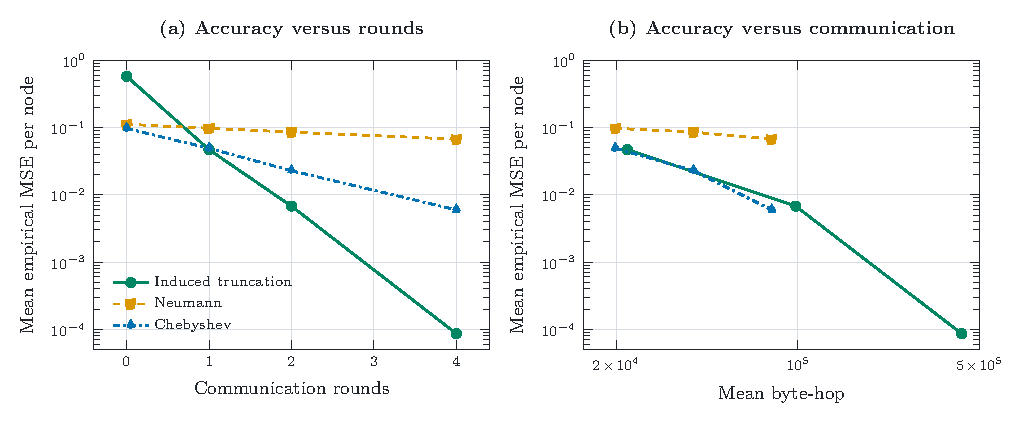
\includegraphics[width=\linewidth]{figures/tikz/local_method_tradeoff.pdf}
  \caption{Fixed-known-graph accuracy and communication tradeoff, averaged
  over four synthetic graph families.  Induced truncation attains the lowest
  error in this small test but collects substantially more model traffic;
  Chebyshev improves much faster than Neumann at the same iterative byte-hop
  count.}
  \label{fig:local-tradeoff}
\end{figure}

\subsection{External scale and accelerator crossover}

The external stress track uses six PGLib-OPF v23.07 networks as weighted
topologies~\cite{babaeinejadsarookolaee2019pglib} and three matrices from the
SuiteSparse Matrix Collection as symmetric sparsity
graphs~\cite{davis2011suitesparse}.  In every case the benchmark constructs the
unit-grounded matrix $I+L$; it does not claim to reproduce the source dataset's
original estimator.  The largest case has 129,164 vertices.  All global
sparse-reference solves meet the configured residual tolerance.
Figure~\ref{fig:external-stress} records the 16-round Chebyshev signal error
and reference-solve time without converting either into a theorem-matched
completion certificate.

\begin{figure}[t]
  \centering
  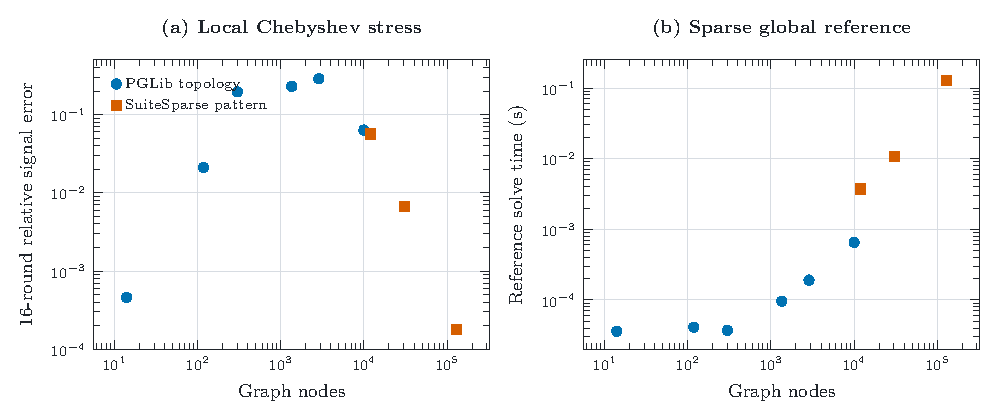
\includegraphics[width=\linewidth]{figures/tikz/external_stress.pdf}
  \caption{External graph-smoother stress tests.  PGLib cases contribute
  topology and positive branch weights; SuiteSparse cases contribute sparsity
  graphs.  Panel (a) reports 16-round Chebyshev relative signal error and panel
  (b) the sparse global-reference solve time.}
  \label{fig:external-stress}
\end{figure}

Finally, three independent process runs compare 40 rounds of a fixed local
Richardson smoother on two-dimensional grids.  The environment fixes OpenMP
and OpenBLAS to one CPU thread and uses an NVIDIA RTX 5080.  Median resident
kernel speedups (CPU time divided by GPU time) are $0.273$, $1.468$, $3.235$,
and $69.38$ at 10,000, 50,176, 102,400, and 1,000,000 states.  Including vector
host--device transfers gives $0.259$, $1.400$, $2.922$, and $50.35$.  Thus the
observed crossover lies between 10,000 and 50,176 states on this system;
wall-clock values are hardware-specific and are not theoretical complexity
claims.

\begin{figure}[t]
  \centering
  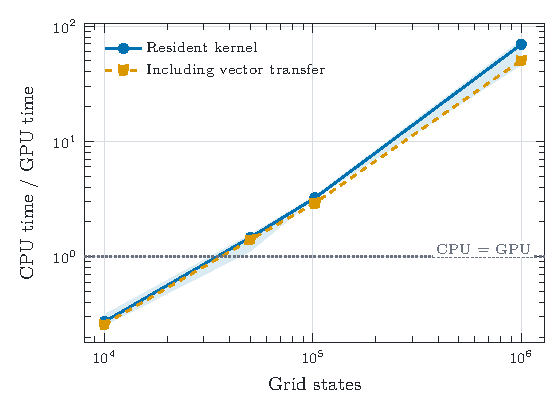
\includegraphics[width=0.58\linewidth]{figures/tikz/cpu_gpu_crossover.pdf}
  \caption{CPU/GPU crossover for a 40-round unit-grounded grid smoother.
  Curves show medians over three process runs, and the blue band spans the
  observed resident-kernel range.}
  \label{fig:cpu-gpu}
\end{figure}

\section{Claim boundaries and relation to prior work}

The following boundaries are part of the result rather than optional
qualifications.

\begin{itemize}[leftmargin=1.5em]
\item Finite-$h$ equality assumes scalar undirected nonnegative edges and unit
grounding.  A uniform finite upper bound on conductance can destroy the
high-conductance converse, and a positive lower bound on connecting edges can
destroy weak-link separation.
\item Hidden-input columns cannot be discarded.  For finite scenarios they
produce $C(X-X^2)C^T$ in \eqref{eq:gram-identity}.
\item The unbounded partial-partition reduction for full errors is sharp at
Schatten exponent two.  It is not a theorem for arbitrary convex losses of the
full error matrix, and it fails for every Schatten exponent below two.
\item The estimator in \eqref{eq:smoother} is graph-regularized state
smoothing.  A raw WLS measurement-noise transfer includes the measurement
operator as an additional right factor; its MSE is not
$\norm{\cA_G(Q)}_F^2$ without a separate derivation.
\item The theorem does not cover directed, signed, block-noncommutative, or
nonlinear completion models.
\end{itemize}

The grounded matrix-forest expansion is classical
\cite{chebotarev1997}.  Pilavci et al.\ explicitly represent graph Tikhonov
regularization as an expectation of random-spanning-forest component averages
\cite{pilavci2021}; general mean-projection identities also appear in
\cite{derezinski2020,kassel2023}.  Full normalized partition matrices and
their polyhedral geometry are studied in clustering
\cite{derosa2022}.  Kron reduction concerns a closely related boundary
elimination operation \cite{dorfler2013}, while boundary groves and electrical
compactifications provide important neighboring partition structures
\cite{kenyon2011,lam2018}.  These works must be cited for the ingredients and
nearby geometry.  Our limited literature search did not locate the combined
finite-hidden-budget hull, complete exposed-vertex rule, connected path
converse, full-input robust reduction, and local-rule SDP stated here.  This is
an ``as far as we are aware'' statement, not a claim that the foundational
forest identity is new or a proof of global priority.

\section{Reproducibility}

The reference implementation is in \texttt{hidden\_completion/}.  The command
\begin{verbatim}
python -m hidden_completion solve <config.json>
\end{verbatim}
accepts $C$, $q$, $h$ (or unbounded mode), and affine local-rule constraints;
it returns $Q$, the re-evaluated exact radius, all active worst-case scenarios,
scenario counts, and separate generation/model/solve timings.  Deterministic
tests cover Bell and Stirling counts, hidden-budget allocation enumeration,
the $X-X^2$ Gram term, exact vertex pruning, $r$-hop masks, shared
coefficients, and the analytic values in \eqref{eq:finite-example} and
\eqref{eq:shared-example}.

The application and figure-data commands are
\begin{verbatim}
python -m experiments.smoother --config <config.json> --output <result.json>
python -m experiments.smoother.paper_data --p3-p4 <result.json> ...
\end{verbatim}
The committed records preserve normalized configurations, RNG seeds, platform
and package versions, source hashes, solver checks, and independent GPU timing
repetitions.  Standalone TikZ/PGFPlots sources, their CSV inputs, vector PDFs,
PNG previews, and the visual-QA record are in
\texttt{paper/figures/tikz/}.

\section{Conclusion}

Unknown hidden topology need not be sampled or replaced by a full-block
uncertainty set for this graph smoother.  Set partitions and hidden-budget
allocations give an exact finite description, including the complete hidden
input, while connected paths certify that every retained boundary scenario is
genuinely sharp.  The result supplies a lossless SDP for constrained common
local rules and an exact budget-to-unbounded convergence rate.  The next step
is not to enlarge the theory class, but to expand the preregistered experiment
matrix, repeat timings across systems, and refine presentation of the exact
certificates and fixed-graph resource tradeoffs.

\bibliographystyle{plain}
\bibliography{references}

\end{document}
